% Universidade Aberta
% Template TeX para relatório de trabalhos
% 2024
%
%
% Dados para a capa
\newcommand{\Titulo}{Diagramas de Componentes Git Activity Provider\\Padrões de Comportamento}
\newcommand{\Ano}{2025}
\newcommand{\Autor}{Hugo Gonçalves}
%
%
\documentclass[12pt,a4paper,final]{article}
\usepackage[stretch=10]{microtype}
\usepackage{csquotes}
\usepackage[portuguese]{babel}
\usepackage{polyglossia}
\setdefaultlanguage{portuguese}
\usepackage{graphicx}
\graphicspath{ {./images/} }
\usepackage[a4paper,top=3cm,bottom=3cm,left=3.5cm,right=2cm]{geometry}
\usepackage{booktabs}
\usepackage{newtxtext}
\usepackage{newtxmath}
\usepackage[pdfauthor=\Autor,
    pdftitle=\Titulo,
    colorlinks=true,
    linkcolor=black,
    citecolor=black,
    bookmarksopen=true]{hyperref}
\hypersetup{colorlinks, citecolor=black, urlcolor=black}
\usepackage{bookmark}
\usepackage{float}
\usepackage{tikz, tikz-uml}
\usepackage[style=apa, backend=biber, sortcites, url=true]{biblatex}
\addbibresource{ref.bib}
\renewcommand{\baselinestretch}{1.5}
\begin{document}
    \title{\Titulo}
    \author{\Autor}
    \date{\Ano}
    \pagenumbering{gobble}
    \begin{titlepage}
        \begin{center}
            \vspace*{4cm}

            \textbf{\large UNIVERSIDADE ABERTA}

            \textbf{\large UNIVERSIDADE DE TRÁS-OS-MONTES E ALTO DOURO}

            \vspace{1cm}

            \begin{minipage}{0.4\textwidth}
                \centering
                
\includegraphics[width=0.8\textwidth]{uab}
            \end{minipage}
            \begin{minipage}{0.4\textwidth}
                \centering
                
\includegraphics[width=0.8\textwidth]{utad}
            \end{minipage}

            \vspace{1.5cm}

            \textbf{\large \Titulo}

            \vspace{1.5cm}

            \textbf{\large \Autor}

            \vspace{2cm}

            \textbf{\large Mestrado em Engenharia Informática e Tecnologia Web}
            \vfill
            \textbf{\Ano}
        \end{center}
    \end{titlepage}
    \renewcommand{\contentsname}{Índice}
    \cleardoublepage
    \pagenumbering{roman}
    \listoffigures
    \newpage
    \cleardoublepage
    \pagenumbering{arabic}

    \noindent O \textit{Git Activity Provider} utiliza o padrão de comportamento \textit{Strategy} no componente Git para abstrair a interação com as diferentes APIs públicas dos repositórios centralizados como GitHub, GitLab, etc.
    Assim, é possível que o \textit{Git Activity Provider} forneça métricas para diferentes repositórios centralizados.
    De acordo com \cite{gamma_1994_design}, o padrão de comportamento \textit{Strategy}, é utilizado para definir uma familia de algoritmos, encapsulando cada um, e tornando-os intercambiáveis.
    A \textit{Strategy} permite que o algoritmo a usar varie independentemente de quem o utiliza.

    \begin{figure}[H]
        \centering
        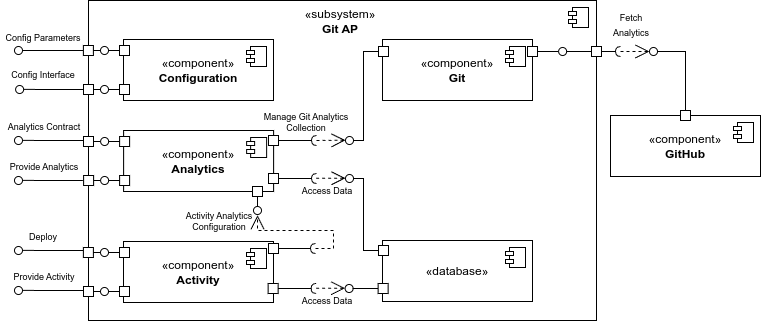
\includegraphics[width=\textwidth]{diagrama_componentes_v2-AP.drawio}
        \caption{Diagrama de Componentes}
        \label{fig:diagrama-componentes}
    \end{figure}

    \noindent Quando um \textit{Active Agent} acede pela primeira vez a uma atividade e define o URL do repositório onde irá desempenhar a atividade, é despoletada uma validação para garantir que o AP dispõe de uma \textit{Strategy} para obter métricas para o repositório indicado pelo \textit{Active Agent}.
    O diagrama representado na figura \ref{fig:diagrama-sequencia} demonstra como esta validação acontece.

    \begin{figure}[H]
        \centering
        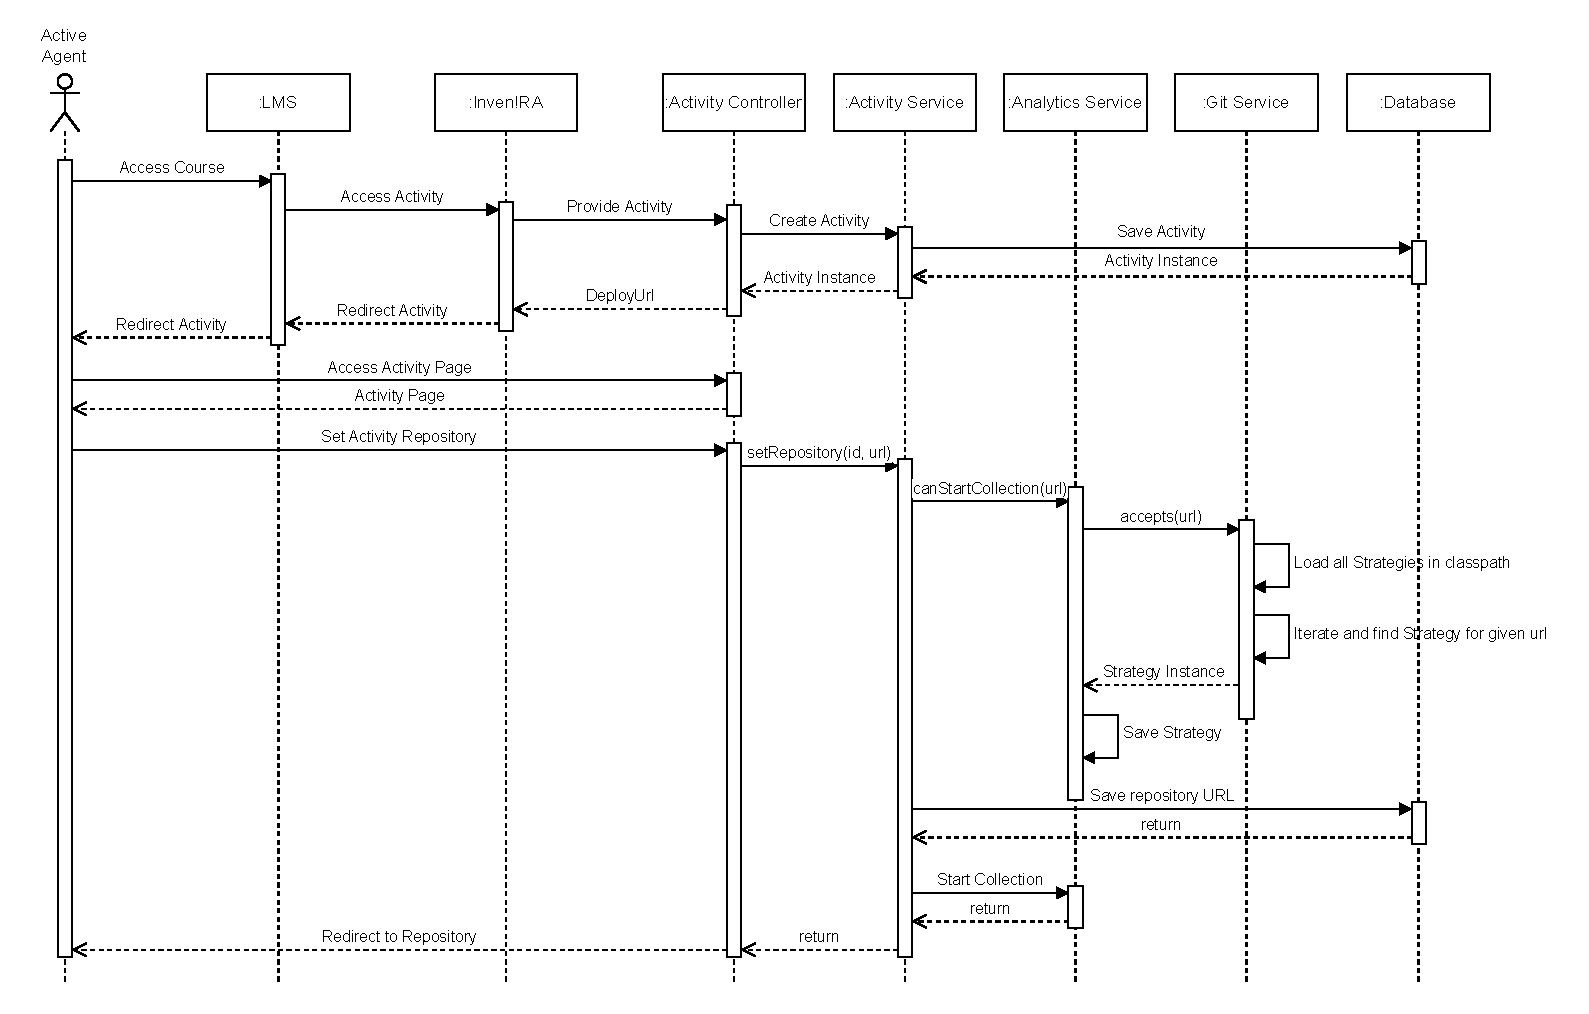
\includegraphics[width=\textwidth]{diagramas_sequencia.drawio}
        \caption{Diagrama de Sequência - \textit{Strategy}}
        \label{fig:diagrama-sequencia}
    \end{figure}
    \newpage
    \printbibliography
\end{document}
